
%%%%%%%%%%%%%%%%%%%%%%%%%%%%%%%%%%%%%%%%%%%%%%%%%%%%%%%%%%%%%%%%%%%%%%%%%%%%%%%%
%%%%%%%%%%%%%%%%%%%%%%%%%%%%%%%%%%%%%%%%%%%%%%%%%%%%%%%%%%%%%%%%%%%%%%%%%%%%%%%%
% OBJETIVOS %
%%%%%%%%%%%%%%%%%%%%%%%%%%%%%%%%%%%%%%%%%%%%%%%%%%%%%%%%%%%%%%%%%%%%%%%%%%%%%%%%

\cleardoublepage % empezamos en página impar
\chapter{Objectives} 
\label{chap:objectives} 

In this chapter, the considered objectives throughout this project are described. In addition, a temporal plan by means of Gantt Chart is included in order to detail the time which has been dedicated to each of them.

\section{General objective}
\label{sec:general-objective}

The objective of this project is to adapt the design and development of the web tool Dr. Scratch to the new version of the programming language Scratch, to analyze the bad practice in the code detected with Dr. Scratch, to implement a new model of visualization for these bad habits and, finally, to evaluate the effectiveness and impact of this model.



\section{Specific objectives}
\label{sec:specific-objectives}

It is important to detail the starting point of the project in order to describe what specific objectives were necessary to achieve the general objective proposed. 

At the beginning of the project, a version of Dr. Scratch already existed. That version analyzed Scratch 2.0 projects and returned different dashboards with the results. However, the work team of Scratch started to announce the launch of a new version of their language in the coming months. 

From this point, the specific objectives were the following:


\begin{itemize}
    \item Documentation and training about the work context: computational thinking, Scratch, Dr. Scratch, bad habits in programming and additional tools. 
    \item To launch the existing version of Dr. Scratch: the version of Django was obsolete. It was necessary to update Django in order to start working with Dr. Scratch. 
    \item To update the code: to remove the modules Hairball and Kurt. For this objective, it was necessary the development of some scripts with the same functionality and the integration of them in the code of Dr. Scratch.
    \item To add new languages: to include the Russian language as an option in the new version of Dr. Scratch.
    \item To create a testing platform in production: to launch a first version of the Dr. Scratch update in a testing platform in Azure, during a month, and to correct possible mistakes during this period.
    \item To coordinate both versions of Dr. Scratch: to have both versions of Dr. Scratch in the same platform of Azure, working in a compatible way in the official web of Dr. Scratch.
    \item To stabilize and maintain the new version: to correct errors and to improve some functionalities.
    \item To collect data and to create the files for a preliminary analysis of bad smells: in order to initiate the analysis, it was necessary to analyze a set of projects with Dr. Scratch, as well as a later process of treatment and filtering of the data.
    \item To perform an analysis of bad smells: an exhaustive analysis of the data set of analyzed projects, mainly with Pandas software. 
    \item To present the first results in the TACKLE Congress: a presentation about the results found in the analysis of bad smells.
    \item To improve the analysis of bad smells: to collect new data for a second analysis and to improve the previous.
    \item To improve the functionality of bad smells in Dr. Scratch: To achieve the analysis of a bigger number of cases about bad smells, such as loop dead code, backdrop naming by default, etc.
    \item To implement a new model based on bad smells: to develop a new dashboard in which bad smells are shown in a more visual and clearer way.
    \item To develop an assessment experiment: to compare the statistics of bad smells, before and after of the developed model, to check its effectiveness and impact.
    
\end{itemize}



\section{Temporary planning}
\label{sec:temporary-planning}

This project has been carried out during two full years. In order to organize temporally the proposed objectives, we identified objectives in the short, medium and long term. In this way, the work is divided into five important phases:

\begin{itemize}
    \item Phase 1: Documentation about the context, to understand the code and fix some bugs.
    
    \begin{figure}[h]
    \centering
        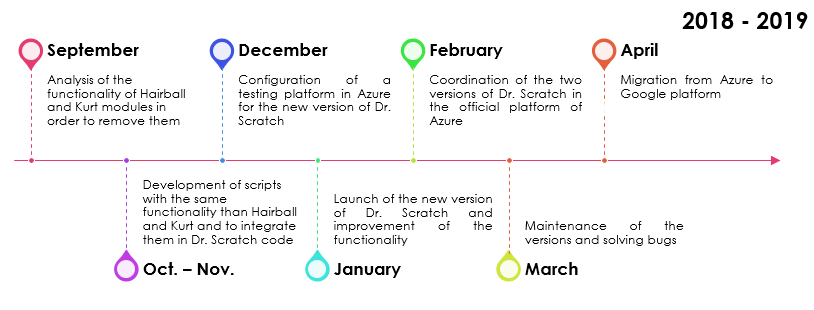
\includegraphics[width=10cm, keepaspectratio]{img/phase_1.png}
        \caption{Temporary planning for Phase 1.}
        \label{fig:phase_1}
    \end{figure}

    \item Phase 2: Update of Dr. Scratch.
    
    \begin{figure}[h]
    \centering
        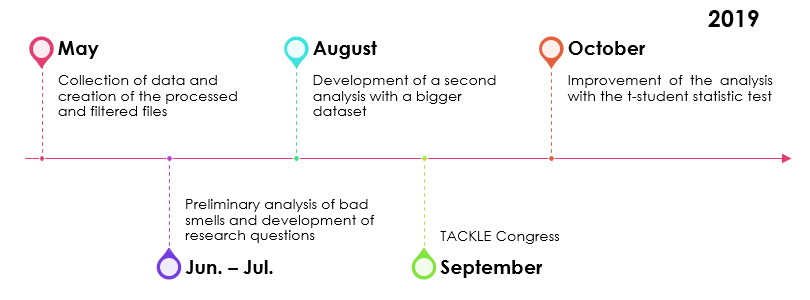
\includegraphics[width=10cm, keepaspectratio]{img/phase_2.png}
        \caption{Temporary planning for Phase 2.}
        \label{fig:phase_2}
    \end{figure}
    
    \item Phase 3: Analysis of bad smells
    
    \begin{figure}[h]
    \centering
        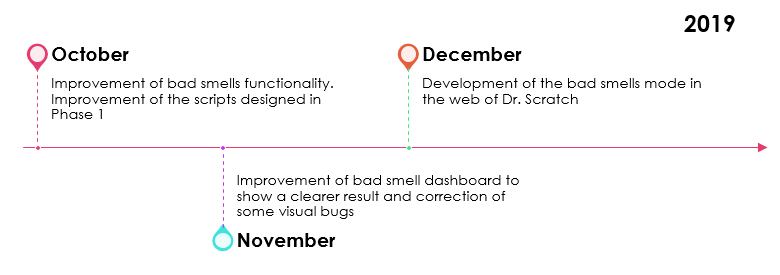
\includegraphics[width=10cm, keepaspectratio]{img/phase_3.png}
        \caption{Temporary planning for Phase 3.}
        \label{fig:phase_3}
    \end{figure}
    
    \item Phase 4: Development of a bad smells model 
    
    \begin{figure}[h]
    \centering
        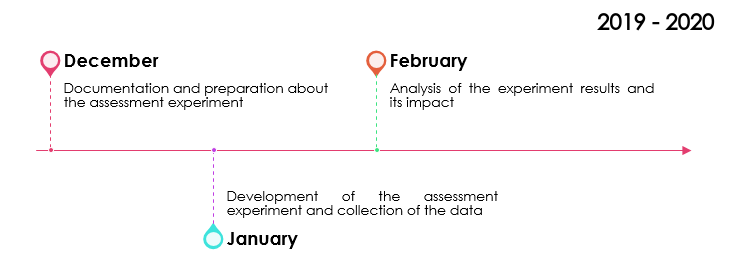
\includegraphics[width=10cm, keepaspectratio]{img/phase_4.png}
        \caption{Temporary planning for Phase 4.}
        \label{fig:phase_4}
    \end{figure}
    
    \item Phase 5: Assessment experiment about the developed model
    
    \begin{figure}[h]
    \centering
        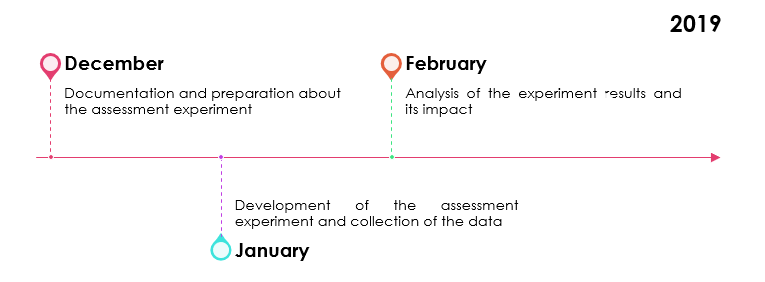
\includegraphics[width=10cm, keepaspectratio]{img/phase_5.png}
        \caption{Temporary planning for Phase 5.}
        \label{fig:phase_5}
    \end{figure}
    
\end{itemize}
